

%\documentclass[12pt]{report}

\documentclass[12pt]{article}
%\usepackage{natbib}  % used for citations
\usepackage[parfill]{parskip} %used for formatting style of text



\usepackage{graphicx,fancyhdr}
\usepackage{amssymb,amsmath}
\usepackage{epigraph,fancyvrb,eqparbox}
\usepackage[multiple]{footmisc}
\usepackage{menukeys}
\usepackage{menukeys}
\usepackage{url}
\usepackage[colorlinks = true, linkcolor = blue, urlcolor = blue]{hyperref}
\usepackage{setspace}

\pagestyle{fancyplain}

%\usepackage{hyperref}
%\usepackage{epsf,psfig,graphicx,fancyheadings}
% \textwidth 7in
% \textheight 9in
% \oddsidemargin 0in
% \topmargin -.25in

%-----------------------------------------------
% The following settings are from Dr. Davidian's
% ST810A Handout on Advanced LaTeX Features

%\setlength{\paperheight}{11.0in}
%\setlength{\paperwidth}{8.5in}

%%%%%%%%%%%%%%%%%%%%%%%%%%%%%%%%%%%%%%%%%%%%%%%%%
% For Desktop @ CalPoly (for Postscript)

%\setlength{\oddsidemargin}{0.5in}
%\setlength{\evensidemargin}{0.5in}
%\setlength{\topmargin}{-.5in}

%%%%%%%%%%%%%%%%%%%%%%%%%%%%%%%%%%%%%%%%%%%%%%%%%
% For Laptop @ Calpoly (for Postscript)

% \setlength{\oddsidemargin}{0.in}
% \setlength{\evensidemargin}{0.in}
% \setlength{\topmargin}{0.25in}

%%%%%%%%%%%%%%%%%%%%%%%%%%%%%%%%%%%%%%%%%%%%%%%%%
% For Desktop @ CalPoly (for PDF)

%\setlength{\oddsidemargin}{0.in}
%\setlength{\evensidemargin}{0.in}
%\setlength{\topmargin}{-.5in}
%
%%%%%%%%%%%%%%%%%%%%%%%%%%%%%%%%%%%%%%%%%%%%%%%%%%
%% For Laptop @ Calpoly (for PDF)
%
%% \setlength{\oddsidemargin}{0.in}
%% \setlength{\evensidemargin}{0.in}
%% \setlength{\topmargin}{0.25in}
%
%
%
%\setlength{\oddsidemargin}{0.0in}
%\setlength{\topmargin}{-0.5in}
%\setlength{\headheight}{0.20in}
%\setlength{\headsep}{3ex}
%\setlength{\baselineskip}{2ex}
%\setlength{\textheight}{9in}
%\setlength{\textwidth}{6.4in}
%\renewcommand{\baselinestretch}{1.1}

% Sets margins to 1 in
\addtolength{\oddsidemargin}{-.5in}%
\addtolength{\evensidemargin}{-.5in}%
\addtolength{\textwidth}{1in}%
\addtolength{\textheight}{1.3in}%
\addtolength{\topmargin}{-.8in}%

%\setlength{\headheight}{0.20in}
%\setlength{\headsep}{3ex}
%\setlength{\headrulewidth}{0.2pt}
%\setlength{\footrulewidth}{0.15pt}
%\setlength{\parskip}{2.3ex}
% %set to no indentation
%\setlength{\parindent}{0.0in}
%\setlength{\baselineskip}{2ex}
%\setlength{\textheight}{9.in}
%\setlength{\textwidth}{6.5in}

\def \doublespace{\openup 2\jot}
% For double or 1.5 spacing
%\renewcommand{\baselinestretch}{1.5}
\tolerance=500

\def\boxit#1{\vbox{\hrule\hbox{\vrule\kern6pt
\vbox{\kern6pt#1\kern6pt}\kern6pt\vrule}\hrule}}
\renewcommand{\theequation}{\thesection.\arabic{equation}}
% The following for TOC
%\renewcommand{\thepage}{\roman{page}}
% to be followed by this for the main text
\renewcommand{\thepage}{\arabic{page}}


%-----------------------------------------------

%%%%%%%%%%%%%%%%%%%%%%%%%%%%%%%%%%%%%%
%Define any shortcut aliases below

\newtheorem{theo}{Theorem}[section]

\newenvironment{note}{\begin{quote}\emph{Note:\ }}{\end{quote}}
\newenvironment{defn}{
\begin{description}
\item[Definition ]}
{\end{description}}

\newenvironment{ttscript}[1]{%
    \begin{list}{}{%
    \settowidth{\labelwidth}{\texttt{#1}}
    \setlength{\leftmargin}{\labelwidth}
    \addtolength{\leftmargin}{\labelsep}
    \setlength{\parsep}{0.5ex plus0.2ex minus0.2ex}
    \setlength{\itemsep}{0.3ex}
    \renewcommand{\makelabel}[1]{\texttt{##1\hfill}}}}
    {\end{list}}

\newcommand{\bt}{\begin{tabular}}
\newcommand{\et}{\end{tabular}}
\newcommand{\bc}{\begin{center}}
\newcommand{\ec}{\end{center}}
\newcommand{\bi}{\begin{itemize}}
\newcommand{\ei}{\end{itemize}}
\newcommand{\be}{\begin{enumerate}}
\newcommand{\ee}{\end{enumerate}}
\newcommand{\bq}{\begin{quote}}
\newcommand{\eq}{\end{quote}}
\newcommand{\vect}[1]{\mbox{\boldmath $ #1$}}
\newcommand{\avg}[1]{$\overline{#1}$}
\newcommand{\bmp}{\begin{minipage}}
\newcommand{\emp}{\end{minipage}}
\newcommand{\hr}{\u{\hspace{7in}}}
\newcommand{\sr}{\u{\hspace{5in}}}
\newcommand{\chs}{\chi^2}

\newcommand{\labn}[1]{\Large{\textbf{\fbox{Lab #1}}}\hspace{0.1in} \normalsize{\emph{Some of these problems may be more challenging than others. Please feel free to work with others, attend office hours, or post on the course discussion forum if you need help.  While collaboration with other students is encouraged, each student is responsible for submitting his or her own work.  This assignment should be submitted in one well-commented SAS program.  For any questions that require a written answer, do so in the SAS comments.  Be sure to re-name the uploaded SAS scripts according to the naming convention}} \texttt{LastnameFirstinitial\textunderscore Lab\#.sas} (\emph{e.g.,} \texttt{PileggiS\textunderscore Lab#1.sas}).}


\newcommand{\hd}[1]{\lhead{STAT 330/530: Lab #1}\rhead{Pileggi, FA17}}
\newcommand{\bs}{\underline{\hspace{0.5in}}}

%\newcommand{\bv}{\footnotesize
%\bmp{.5\textwidth}
%\begin{Verbatim}[frame=single,label=SAS Code,commandchars=\\\{\}],xrightmargin=.5\textwidth}
%
%\newcommand{\ev}{\end{Verbatim}
%\emp
%\normalsize}

\newcommand{\bv}{\begin{code}}
\newcommand{\ev}{\end{code}}

 \newenvironment{code}[1]%
  {\vspace{.1in}\footnotesize\Verbatim[frame=single,label=SAS Code,commandchars=\\\{\},xrightmargin=#1\textwidth,framesep=.2in,labelposition=all]}
  {\endVerbatim\normalsize}

\newenvironment{craw}[2]%
{\vspace{.1in}\footnotesize\Verbatim[frame=single,label=#2,commandchars=\\\{\},xrightmargin=#1\textwidth,framesep=.2in,labelposition=all]}
  {\endVerbatim\normalsize}

\newenvironment{cbox}[1]%
{\vspace{.1in}\footnotesize\Verbatim[frame=single,commandchars=\\\{\},xrightmargin=#1\textwidth,framesep=.2in,labelposition=all]}
  {\endVerbatim\normalsize}

\newcommand{\head}[1]{\large \textbf{#1} \normalsize}

\newcommand{\ttt}[1]{\textbf{\texttt{#1}}}


\newcommand{\bsval}[1]{\underline{\hspace{0.2in}{[#1]}\hspace{0.2in}}}

\newcommand{\ttb}{\textbf}
\newcommand{\tte}{\emph}
\newcommand{\ttu}{\underline}



\newcommand{\jdhr}{\vspace{0.2in}\hrule}


\newcommand{\uspace}[1]{\underline{\hspace{#1}}}

\newenvironment{ident}{\begin{list}{}{}
         \item[]}{\end{list}}

\newenvironment{proposition}{
\begin{description}
\item[Proposition: ]}
{\end{description}}

\newcommand{\bpr}{\begin{proposition}}
\newcommand{\epr}{\end{proposition}}



% \newenvironment{example}
%     {
%         \begin{list}{\textbf{Example:}}
%         {
%         \settowidth{\labelwidth}{}
%         \setlength{\leftmargin}{\labelwidth}
%         }
%     }
%     {\end{list}}


\newenvironment{example}{
\jdhr \vspace{-.17in}\jdhr
\textbf{Example: }}
{}

\newcommand{\bex}{\begin{example}}
\newcommand{\eex}{\end{example}}

\newenvironment{onyourown}{
\jdhr \vspace{-.17in}\jdhr
\textbf{On Your Own: }}
{}

\newcommand{\boy}{\begin{onyourown}}
\newcommand{\eoy}{\end{onyourown}}


%\newenvironment{debug}{
%\jdhr \vspace{-.17in}\jdhr
%\ttb{Debug the Code}
%\fbox{
%\bmp{.95in}
%\includegraphics[height=.35in]{C:/images/bug4.jpg}\includegraphics[height=.35in]{C:/images/buggy8.jpg}
%\emp}
%}
%{\jdhr}

\newenvironment{debug}{
\jdhr \vspace{-.17in}\jdhr
\ttb{Debug the Code: }
\fbox{
\bmp{.95in}
\includegraphics[height=.35in]{C:/images/bug4.jpg}\includegraphics[height=.35in]{C:/images/mushi90.jpg}
\emp}
}
{}


\newcommand{\bbug}{\begin{debug}}
\newcommand{\ebug}{\end{debug}}


\begingroup
  \catcode `_=11
  \gdef\myuscore{_}
  \catcode `~=11
  \gdef\mytilde{~}
  \catcode `\|=0
  \catcode `\\=11
  |gdef|mybs{\}
|endgroup

%Define any shortcut aliases above


%....................................................................
%....................................................................
%....................................................................
%....................................................................
%....................................................................
%....................................................................
%....................................................................
%....................................................................



\usepackage{amssymb}
				

\begin{document}
\hd{14}
\labn{14}
\vskip10pt
\vskip10pt
\begin{enumerate}
\item Create a SAS library to access the \ttt{O2012.sas7bdat} data set.  This data set is about Olympic medalists from the 2012 Olympics.  Recall that this data set starts with an ``oh'' and not a ``zero''.
\item Write a couple of SAS procedures to help you familiarize yourself with the data and summarize  the data.  How many observations are there?  What does an observation represent?  Note your findings as a comment in your SAS code.
\item Create a new, temporary data set that sorts the olympics data by participating countries.
\item Create a second new, temporary data set.  In this data set, create the following variables.  It may be helpful if you create them in the chunks presented below, then carefully check your data to make sure the variables were created correctly.
\begin{enumerate}
\item medal variables
\item[] \ttt{num\text\_medalists} - total number of medalists for each country
\item[] \ttt{num\_gold} - total number of gold medals for each country
\item[] \ttt{num\_silver} - total number of silver medals for each country
\item[] \ttt{num\_bronze} - total number of bronze medals for each country
\item[] \ttt{num\_total} - total number of medals (gold, silver, and bronze) for each country
\item functions of medals
\item[] \ttt{ave\_medals} - total number of medals divided by total number of medalists for each country (represents average medals earned per medalist)
\item[] \ttt{max\_medals} - maximum number of total medals earned by an \emph{individual} athlete for each country
\item athlete variables
\item[] \ttt{ave\_age}  - average age of all medalists for each country
\item[] \ttt{ave\_wt}  - average weight of all medalists for each country
\item[] \ttt{ave\_ht} -  average height of all medalists for each country
\item[] \ttt{prop\_m}  - proportion of all medalists that are male for each country
\end{enumerate}
\item Carefully examine the \ttt{ave\_medals} variable.
\begin{enumerate}
\item In a comment in your SAS code, explain why it doesn't make sense for a country to have a \ttt{ave\_medals} less than one.
\item Identify the three countries that have \ttt{ave\_medals} less than one.  Note your results in a comment in your SAS code.
\item Print the \ttt{country}, \ttt{name}, \ttt{total}, \ttt{num\_total}, \ttt{num\_medalists} and \ttt{ave\_medals} variables  for these three countries.  Explain how they ended up having a \ttt{ave\_medals} less than one.  Note your findings in a comment in your SAS code. \emph{Note: you do not need to fix or create a cleaned version of this variable.}
\end{enumerate}
\item Similarly to the  \ttt{ave\_medals} variable, the \ttt{ave\_wt} variable was also incorrectly calculated.
\begin{enumerate}
\item Use a SAS procedure to identify the six \emph{sports} in which athletes have missing values for weights.  Note your findings as a comment in your SAS code.
\item Use a SAS procedure to identify which sport has the largest number of missing values for weight.  Note your findings as a comment in your SAS code.
\item Go back to your data step from question 4 and create a new variable that represents the total number of medalists without missing weight values (\ttt{num\_nomisswt}).
\item Calculate a corrected average weight of the athletes for each country (ave\_wt\_fixed) using the new variable from (b).
\item[]\emph{Note: Other variables that have missing values were also calculated incorrectly.  You are not required to fix these other variables.}
\end{enumerate}
\item
Create country level information.
\begin{enumerate}
\item  Create a third temporary data set that only has one observation per country.  This data set should only have the variable \ttt{country} and the variables that you created in questions 4 and 6.
\item Print your data using an option such that a maximum of two decimal places are displayed in the output.  So that you may check your work, a print out for the first 15 countries is provided on the next page (note the output is \emph{wrapping} due to the number of variables).
\end{enumerate}
%\item[]
%\bmp{1.0\textwidth}
%\footnotesize
%\begin{craw}{.0}{Values from final data set}
%                         num_    num_        max_          ave_wt_
%   Obs Country        medalists total ratio medals ave_age  fixed  prop_m
%
%     1 Australia          25      32   1.28    4    24.44   73.16   0.24
%     2 Azerbaijan          1       1   1.00    1    18.00   56.00   1.00
%     3 Belarus             4       4   1.00    1    29.50   68.25   0.25
%     4 Belgium             2       2   1.00    1    26.00   61.00   0.50
%     5 Brazil              5       5   1.00    1    23.40   81.60   0.60
%     6 Canada             25      25   1.00    1    28.24   77.76   0.44
%     7 Colombia            3       3   1.00    1    26.67   64.67   0.67
%     8 Croatia             4       4   1.00    1    23.50   94.00   1.00
%     9 Cuba                5       5   1.00    1    26.40   78.00   0.60
%    10 Czech Republic      2       2   1.00    1    27.00   85.50   1.00
%\end{craw}
%\emp
\end{enumerate}
\hspace*{-0.3in}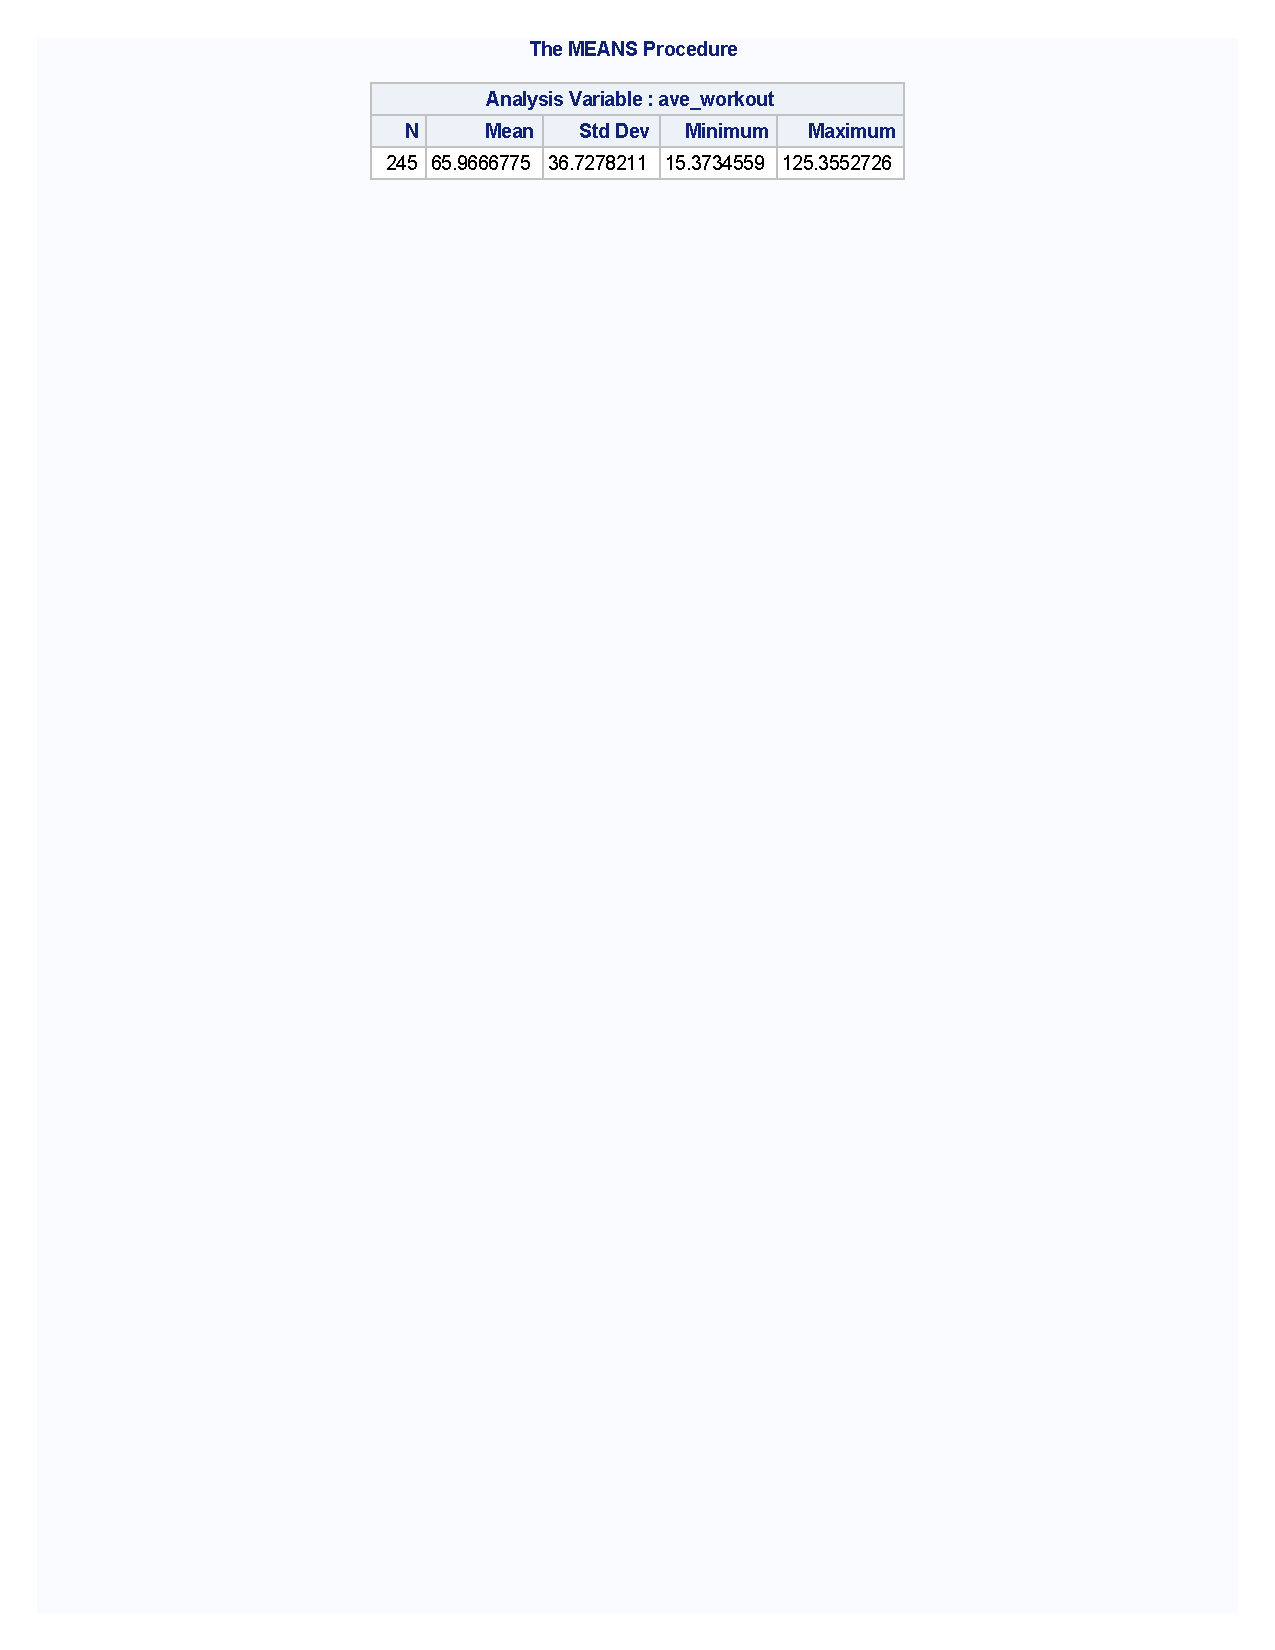
\includegraphics[width=1.0\textwidth]{q7.pdf}
\end{document} 